% !TEX root = perelman-geometry.tex
%!TEX TS-program = pdflatex
%!TEX encoding = UTF-8 Unicode



\setchapterpreamble[o]{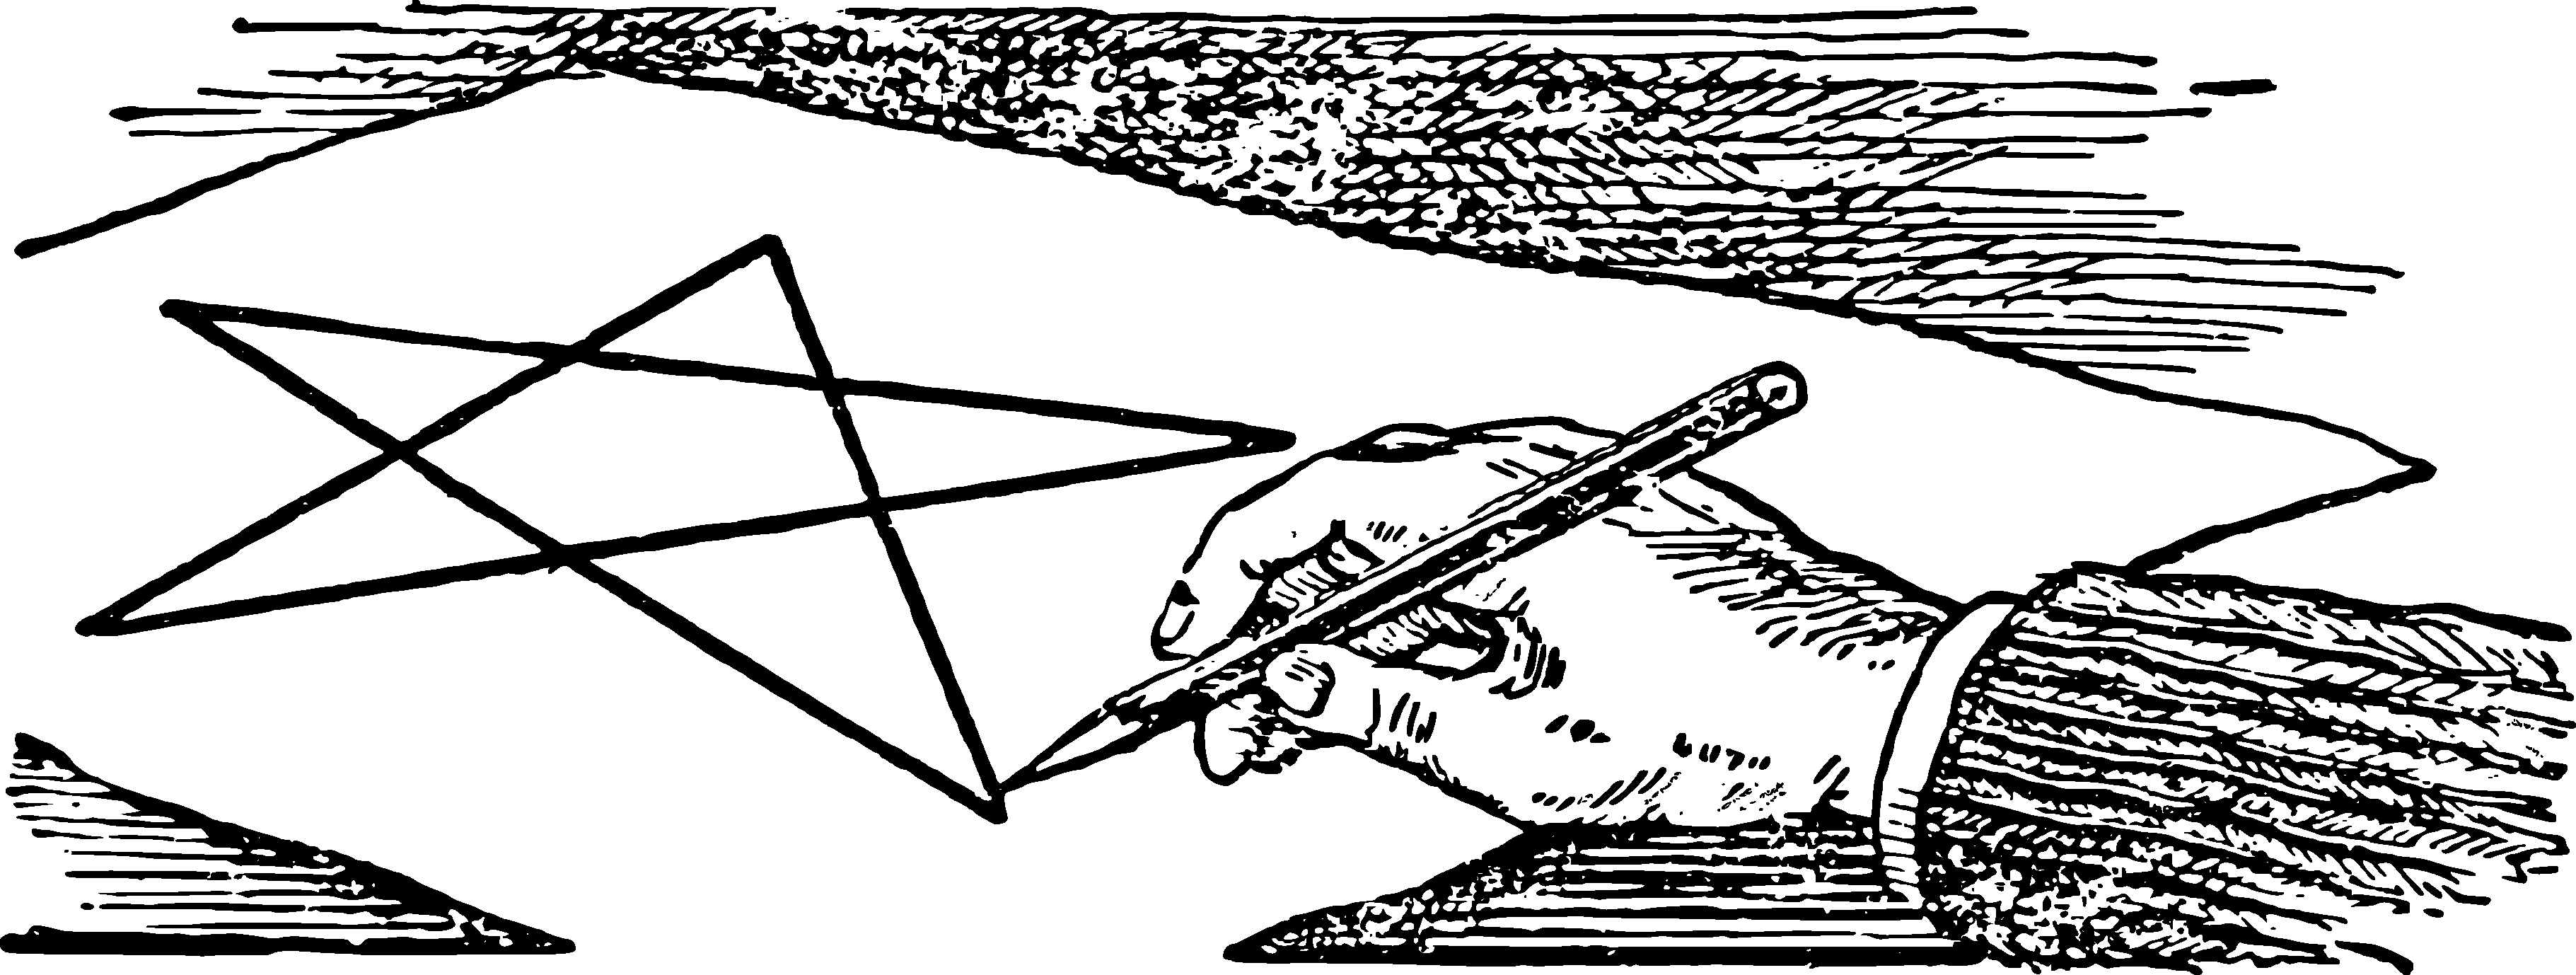
\includegraphics[width=1.2\textwidth]{figures/ch-10/fig-ch-10-head.pdf}\bigskip}

\chapter[Geometry Without Measurements And Calculations]{Geometry Without Measurements And Without Calculations}
\label{ch-10}



\section{Building without a compass}
\label{sec-10.1}

When solving geometric construction problems, rulers and compasses are usually used. However, we will now see that sometimes it is possible to do without a compass in such cases where at first glance it seems absolutely necessary.

\begin{figure}[h!]
\centering
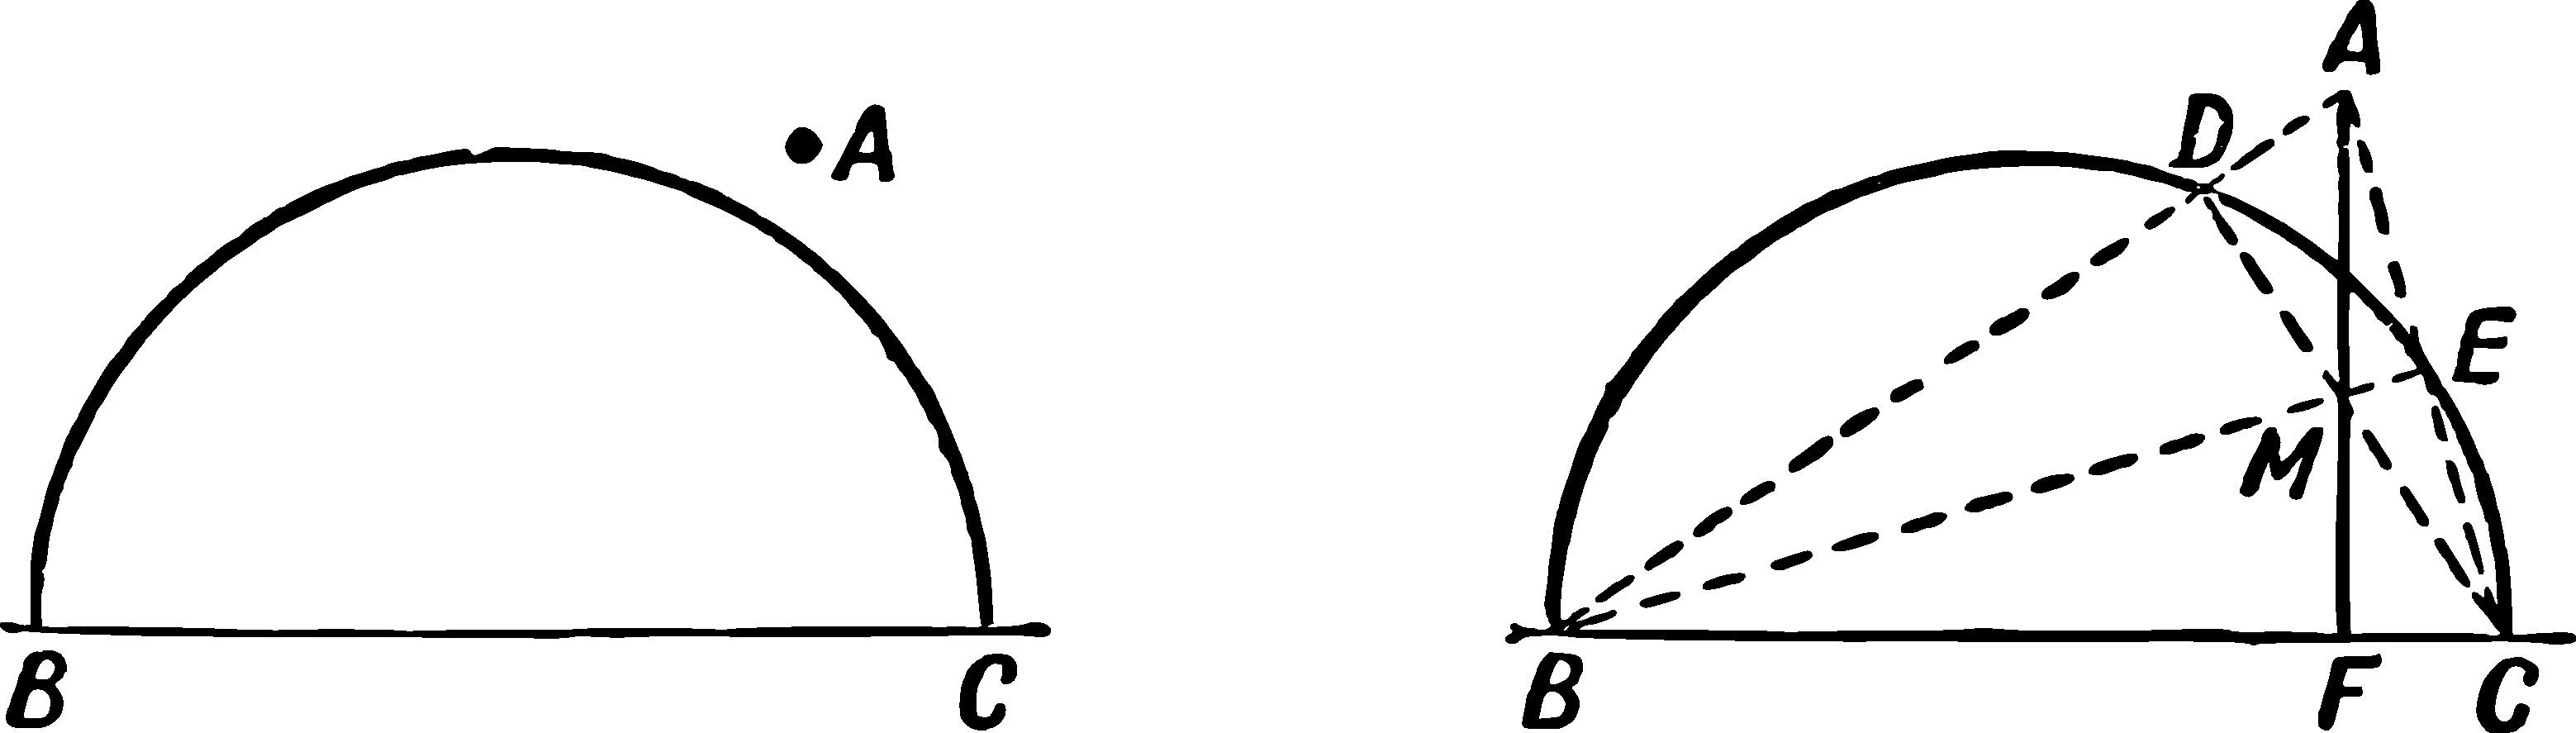
\includegraphics[width=0.9\textwidth]{figures/ch-10/fig-141.pdf}
\sidecaption{The task of building and solving it. The first case.\label{fig-141}}
\end{figure}

\ques From point $A$ (\figr{fig-141}, left), lying outside the given semicircle, drop a perpendicular to its diameter without using a compass. The position of the centre of the semicircle is not indicated.

\ans We will use the property of a triangle that all its altitudes intersect at a single point. Connect $A$ with  $B$ and $C$; we get points $D$ and $E$ (\figr{fig-141}, right). The lines $BE$ and $CD$ are obviously the altitudes of triangle $ABC$. The third altitude, which is the required perpendicular to $BC$, must pass through the intersection point of the other two, i.e., point $M$. By drawing a line through points $A$ and $M$ with a ruler, we meet the requirements of the task without using a compass. 

\begin{figure}[h!]
\centering
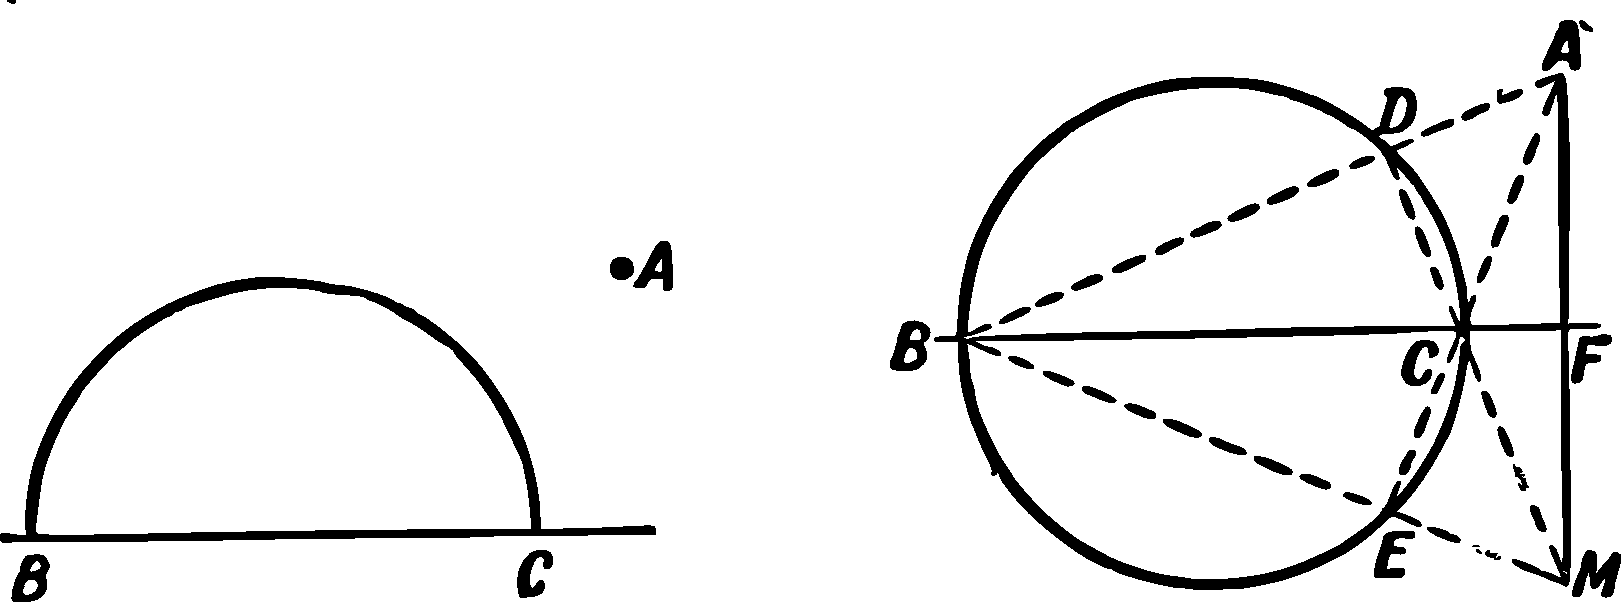
\includegraphics[width=0.9\textwidth]{figures/ch-10/fig-142.pdf}
\sidecaption{The same task. Second case.\label{fig-142}}
\end{figure}


If the point is positioned such that the required perpendicular falls on the extension of the diameter (\figr{fig-142}), then the problem is solvable only if a full circle, rather than a semicircle, is given. \figr{fig-142} shows that the solution is no different from the one we are already familiar with; only the altitudes of triangle $ABC$ intersect not inside, but outside of it.


\section{Centre of Gravity of a Plate}
\label{sec-10.2}

\begin{marginfigure}[-1cm]%[h!]
\centering
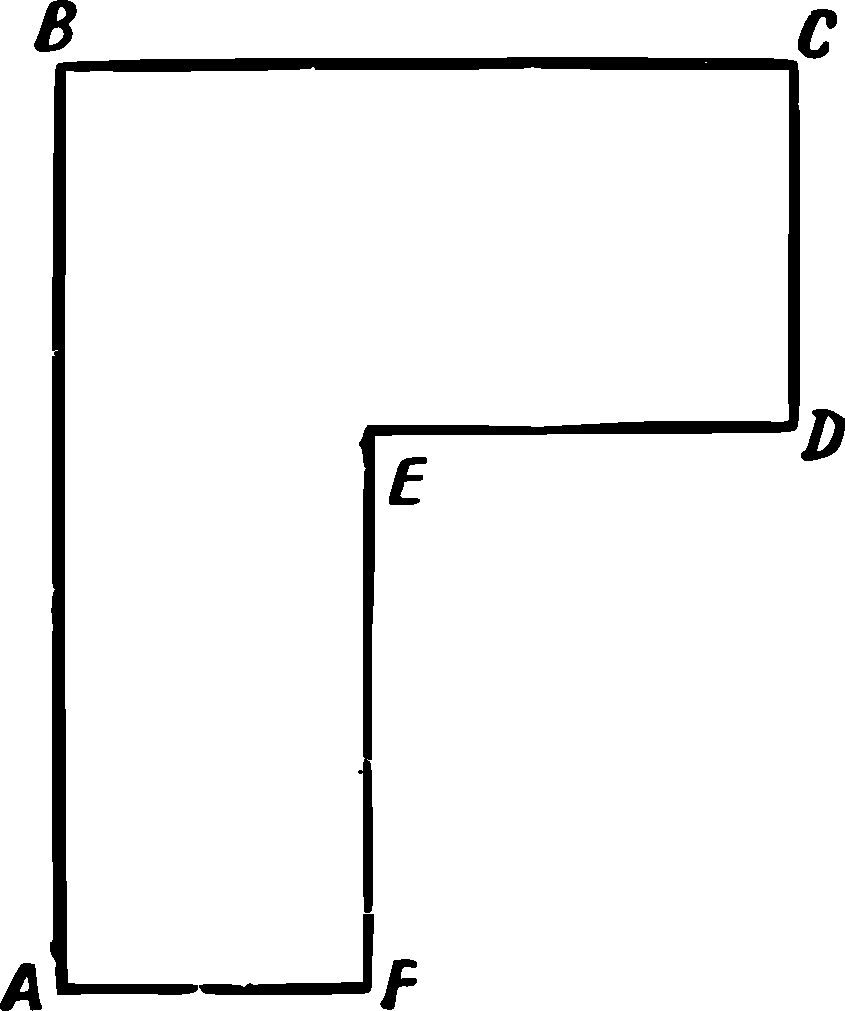
\includegraphics[width=\textwidth]{figures/ch-10/fig-143.pdf}
\sidecaption{Using only a ruler, find the centre of gravity of the depicted plate.\label{fig-143}}
\end{marginfigure}


\ques You probably know that the centre of gravity of a thin, uniform plate, which has the shape of a rectangle or a rhombus, is located at the intersection of the diagonals, and if the plate is triangular, it is at the intersection of the medians. If the plate is circular, it is at the centre of the circle.





Now try to figure out how to find the centre of gravity of a plate made up of two arbitrary rectangles joined into one shape, as shown in \figr{fig-143}. Let's agree to use only a ruler and not to measure or calculate anything.


\ans Extend side $DE$ to intersect with $AB$ at point $N$ and side $FE$ to intersect with $BC$ at point $M$ (\figr{fig-144}). We will first consider the given figure as composed of the rectangles $ANEF$ and $NBCD$. The centre of gravity of each of them is at the intersection points of their diagonals, $O_{1}$ and $O_{2}$.


\begin{marginfigure}%[h!]
\centering
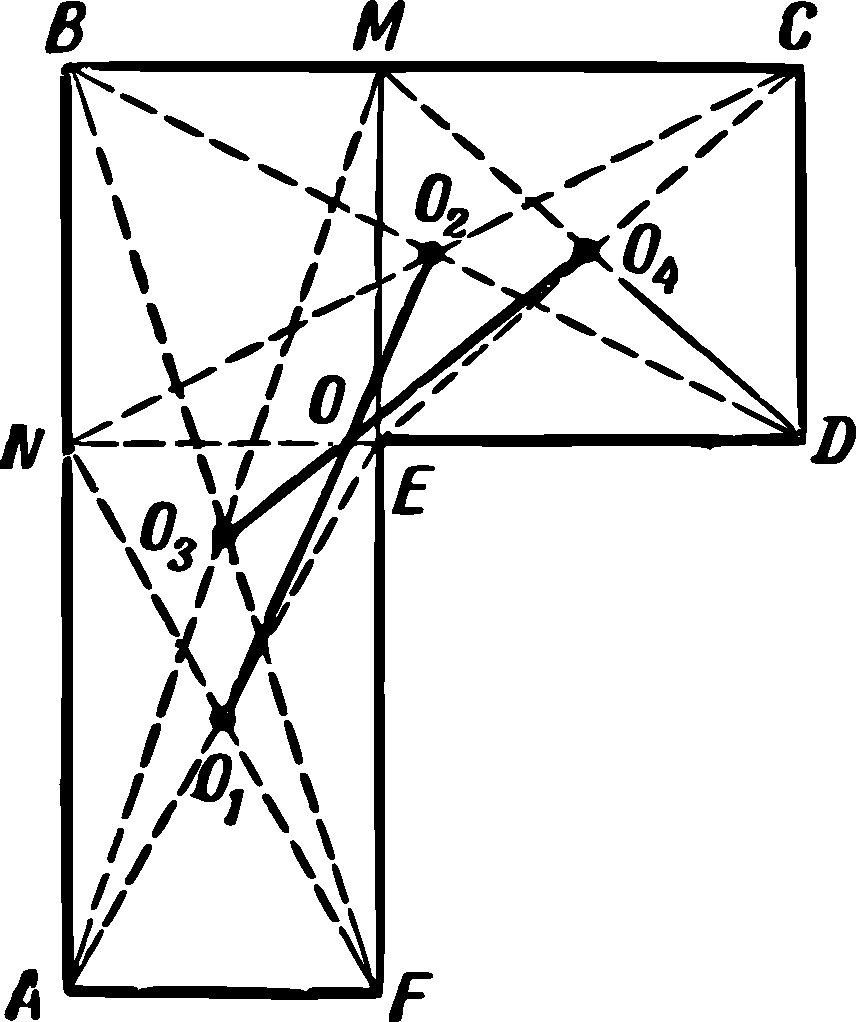
\includegraphics[width=\textwidth]{figures/ch-10/fig-144.pdf}
\sidecaption{The centre of gravity of the plate found.\label{fig-144}}
\end{marginfigure}


Therefore, the centre of gravity of the entire figure lies on the line $O_{1}O_{2}$. Now, consider the same figure as composed of the rectangles $ABMF$ and $EMCD$, whose centres of gravity are at the intersection points of their diagonals, $O_{3}$ and $O_{4}$. The centre of gravity of the entire figure lies on the line $O_{3}O_{4}$. Hence, it lies at the point $O$ where the lines $O_{1}O_{2}$ and $O_{3}O_{4}$ intersect. All these constructions are indeed carried out only with the help of a ruler.






\section{Napoleon's Task}
\label{sec-10.3}


We have just been dealing with a construction performed using only a ruler, without resorting to a compass (on the condition that one circle is given in the drawing in advance). Now let us consider several problems in which the opposite restriction is introduced: the use of a ruler is prohibited, and all constructions must be performed using only a compass. One such problem interested Napoleon (who, as is well known, was interested in mathematics). After reading a book on such constructions by the Italian scientist Mascheroni, he posed the following problem to French mathematicians:

\ques Divide a given circle into four equal parts without using a ruler. The position of the centre of the circle is given.


\begin{marginfigure}%[h!]
\centering
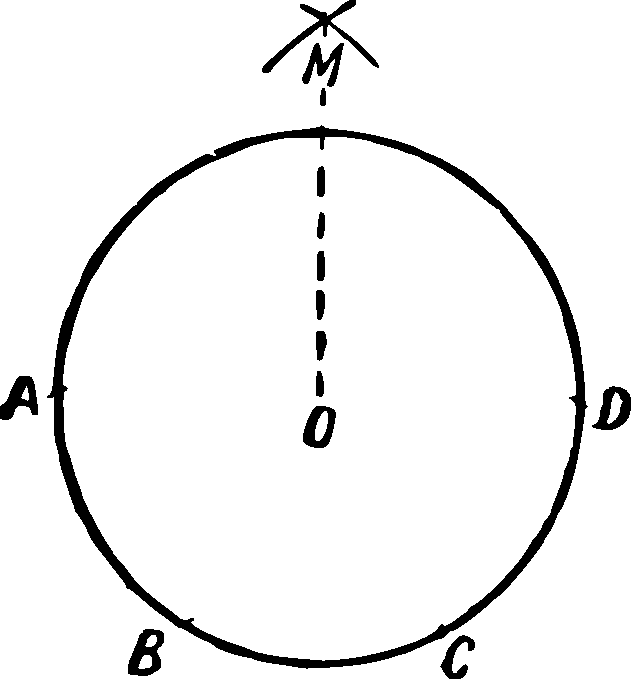
\includegraphics[width=\textwidth]{figures/ch-10/fig-145.pdf}
\sidecaption{Divide the circle into four equal parts using the ruler.\label{fig-145}}
\end{marginfigure}


\ans Suppose we need to divide circle $O$ (\figr{fig-145}) into four parts. From an arbitrary point $A$, we lay off three times the radius of the circle along the circumference: we obtain points $B$, $C$, and $D$. It is easy to see that the distance $AC$, the chord of the arc constituting 1/3 of the circle, is the side of the inscribed equilateral triangle and therefore equals \( r \sqrt{3} \), where \( r \) is the radius of the circle. $AD$ is obviously the diameter of the circle. From points $A$ and $D$, with a radius equal to $AC$, we draw arcs intersecting at point $M$. We will show that the distance $MO$ is equal to the side of the square inscribed in our circle. In triangle $AMO$, the leg $MO$ equals \( \sqrt{AM^{2} - AO^{2}} = \sqrt{3r^{2} - r^{2}} = r\sqrt{2} \), i.e., the side of the inscribed square. Now, using the compass set to MO, we lay off four points on the circle in succession to obtain the vertices of the inscribed square, which will obviously divide the circle into four equal parts.


\ques Here is another, easier problem of the same kind. Without a ruler, increase the distance between given points $A$ and $B$ (see \figr{fig-146}) by five times, or more generally, by any given factor.

\begin{marginfigure}%[h!]
\centering
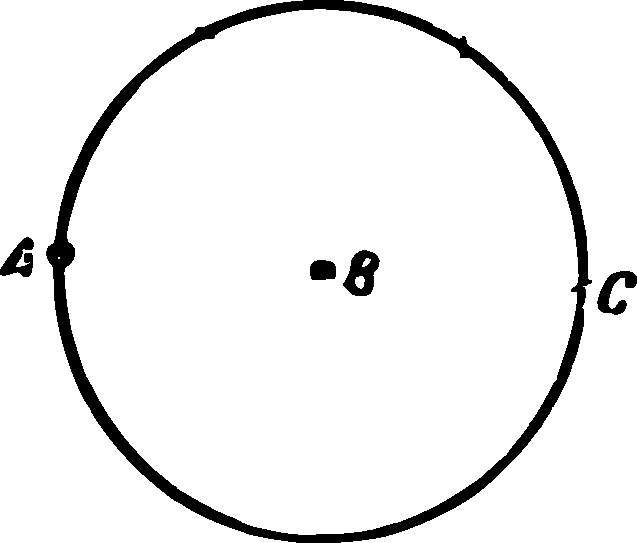
\includegraphics[width=\textwidth]{figures/ch-10/fig-146.pdf}
\sidecaption{How can we increase the distance between points $A$ and $B$ by a factor $n$ (an integer) using only a compass?\label{fig-146}}
\end{marginfigure}

\ans From point $B$, draw a circle with radius $AB$ (see \figr{fig-146}). Along this circle, measure the distance $AB$ three times from point $A$: you get point $C$, which is obviously diametrically opposite to $A$. The distance $AC$ is twice the distance $AB$. By drawing a circle from point $C$ with radius $BC$, we can similarly find a point diametrically opposite to $B$ and, therefore, three times the distance $AB$ from $A$, and so on.


\section{Simple Trisector}
\label{sec-10.4}

Using only a compass and an unmarked ruler, it is impossible to divide an arbitrarily given angle into three equal parts. However, mathematics does not completely rule out the possibility of performing this division using some other devices. Many mechanical devices have been invented to achieve this goal. These devices are called trisectors. You can easily make a simple trisector from stiff paper, cardboard, or thin metal. It will serve as an auxiliary drawing tool.


\begin{figure}[h!]
\centering
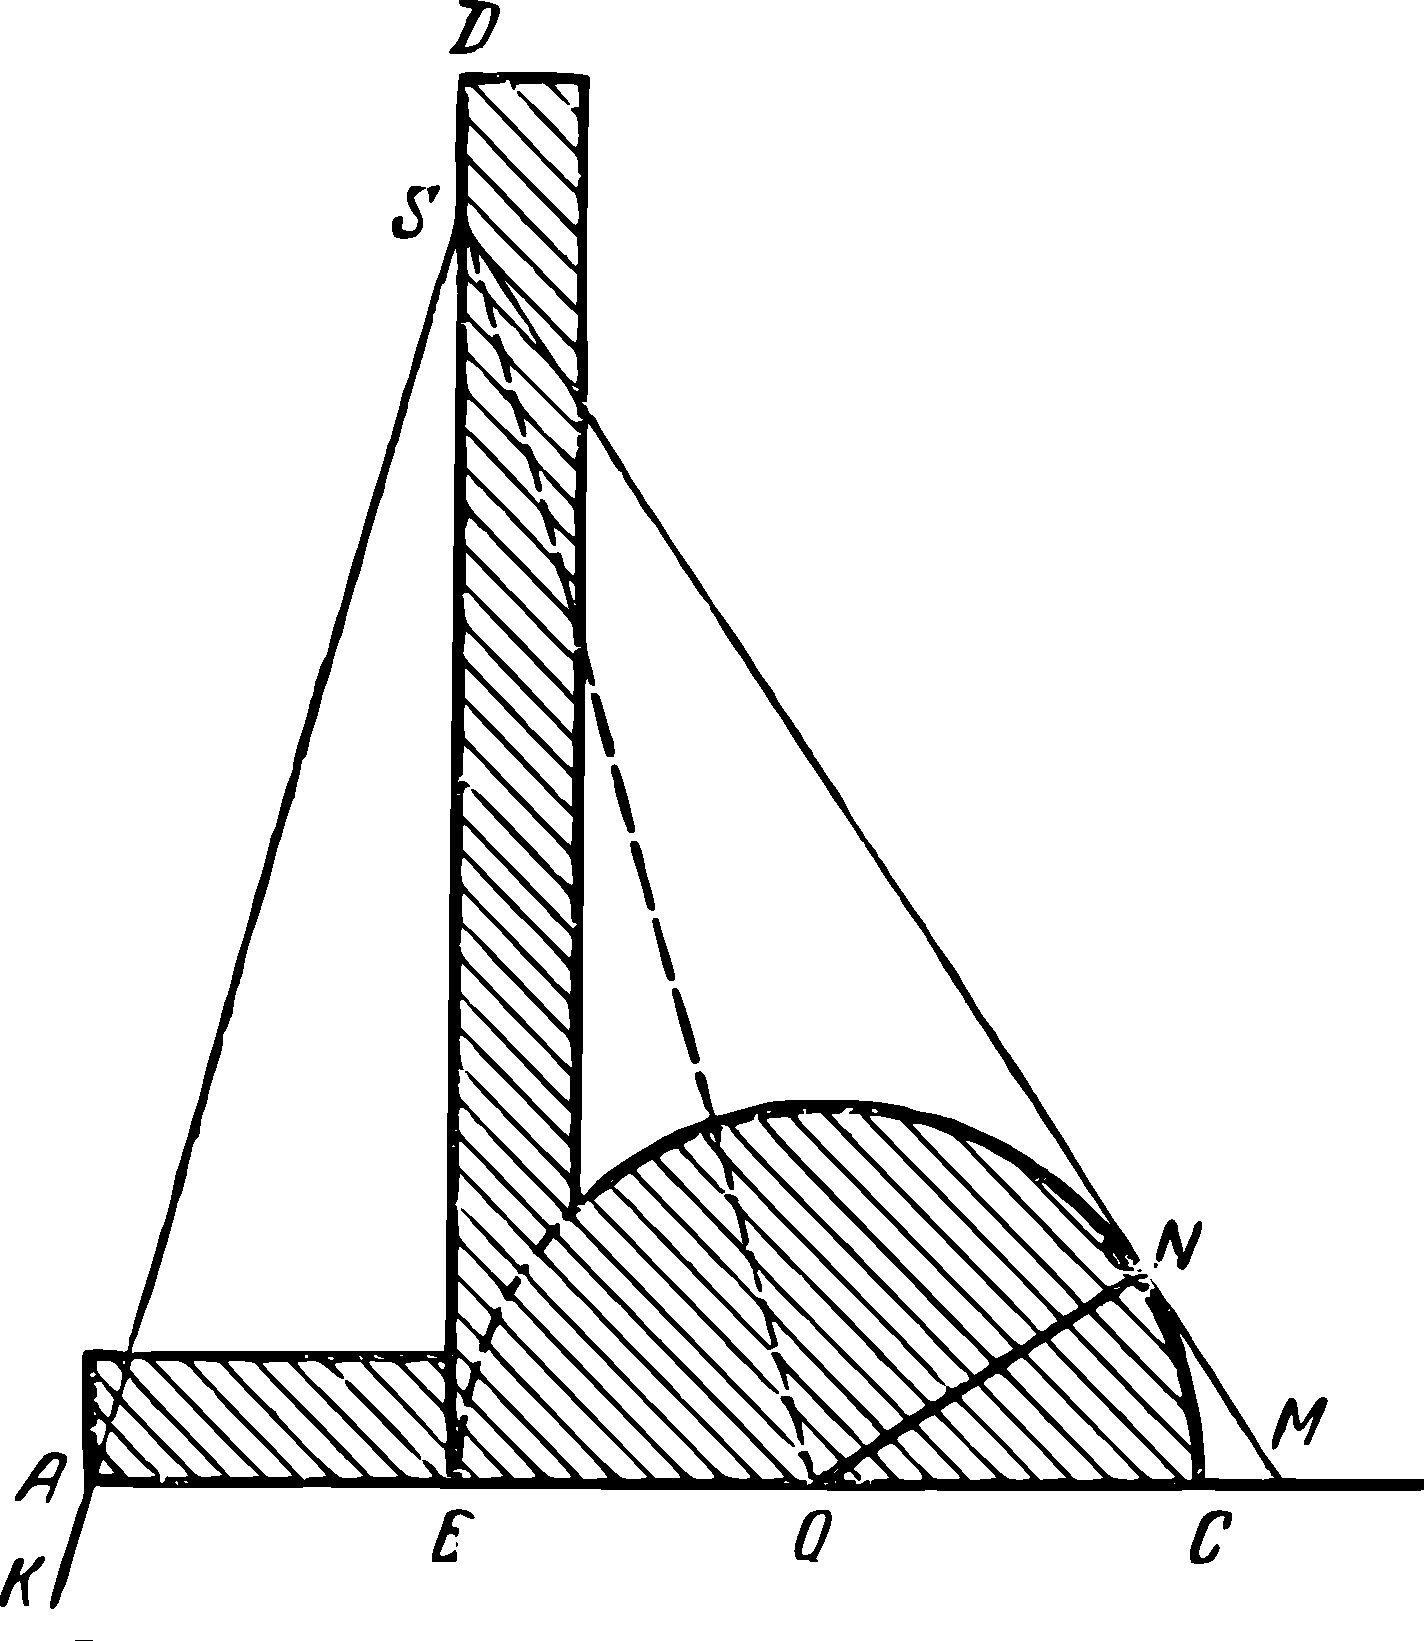
\includegraphics[width=0.8\textwidth]{figures/ch-10/fig-147.pdf}
\sidecaption{Trisector and its usage scheme.\label{fig-147}}
\end{figure}


In \figr{fig-146}, the trisector is shown at full scale (shaded figure). The strip $AB$ adjacent to the semicircle is equal in length to the radius of the semicircle. The edge of the strip $BD$ forms a right angle with the line $AC$; it touches the semicircle at point $B$; the length of this strip is arbitrary. The same figure shows how to use the trisector. For example, let’s say you need to divide the angle $KSM$ (\figr{fig-146}) into three equal parts.

Place the trisector so that the vertex of the angle $S$ is on the line $BD$, one side of the angle passes through point $A$, and the other side touches the semicircle at point\sidenote{The possibility of fitting our trisector into a given angle follows from a simple property of the points on the rays dividing the angle into three equal parts: if from any point $O$ on the ray $SO$ you draw segments $ON \perp SM$ and $OA \perp SB$ (\figr{fig-147}), then we have: $AB = OB = ON$. The reader can easily prove this for themselves.}. Then draw straight lines $SB$ and $SO$, and the division of the given angle into three equal parts is complete. To prove this, connect the centre of the semicircle $O$ to the point of tangency $N$ with a straight line segment. It is easy to see that triangle $ASB$ is equal to triangle $SBO$, and triangle $SBO$ is equal to triangle $OSN$. From the equality of these three triangles, it follows that angles $ASB$, $BSO$, and $OSN$ are equal to each other, which is what was required to be proved.

This method of angle trisection is not purely geometric; it can be called mechanical.


\section{Clock Trisector}
\label{sec-10.5}

\ques Is it possible to divide a given angle into three equal parts using a compass, a ruler, and a clock?

\ans Yes, it is possible. Transfer the figure of the given angle onto transparent paper and, at the moment when both clock hands overlap, place the drawing onto the clock face so that the vertex of the angle coincides with the centre of the clock hands' rotation and one side of the angle aligns with the hands (\figr{fig-148}).

\begin{figure}[h!]
\centering
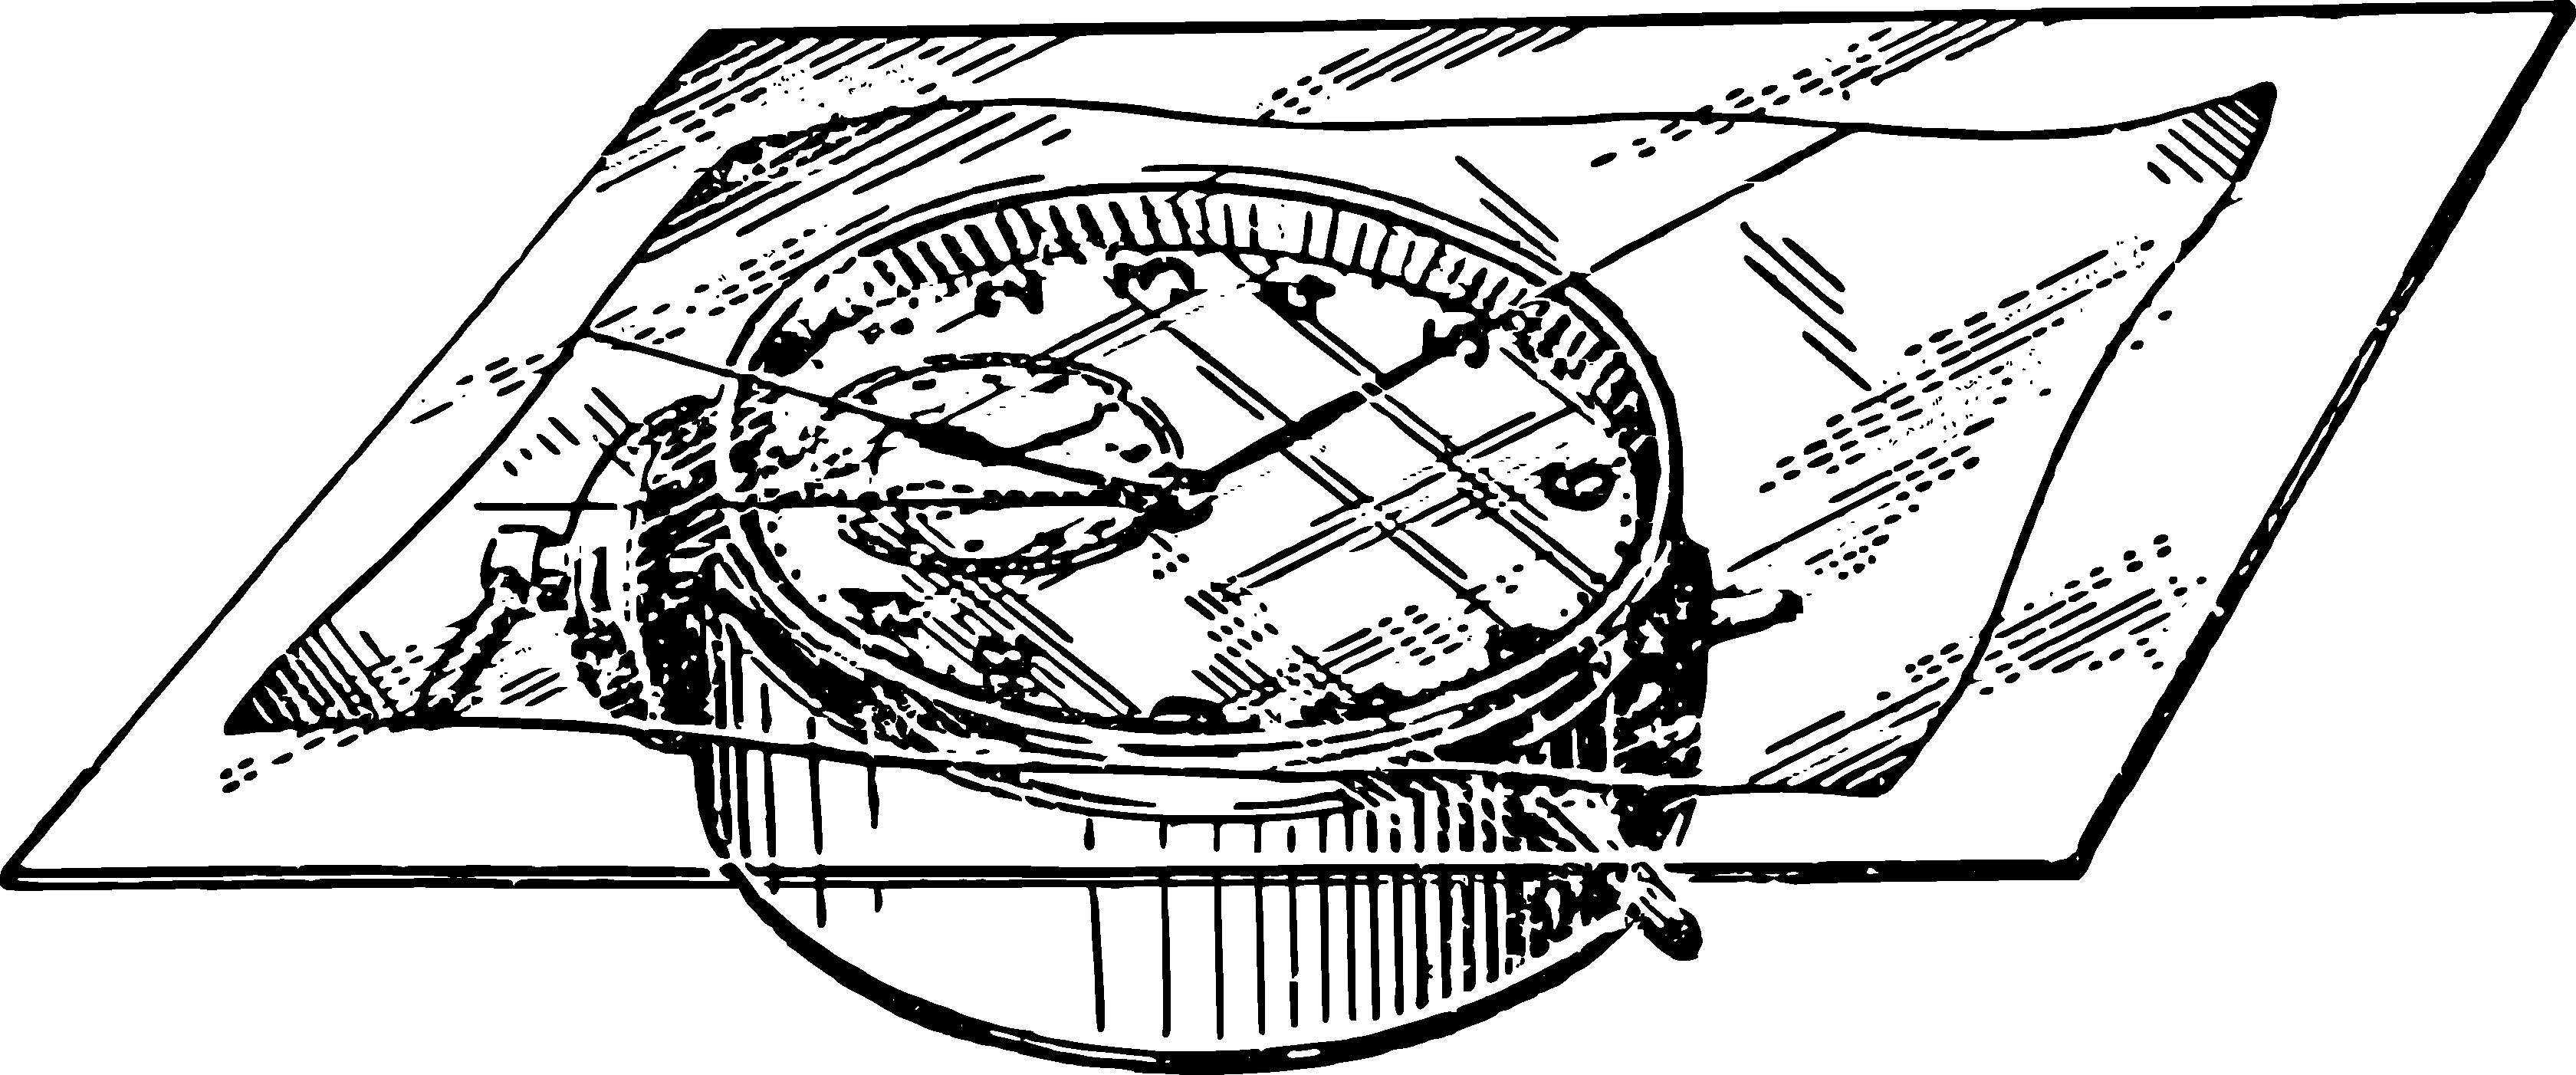
\includegraphics[width=0.85\textwidth]{figures/ch-10/fig-148.pdf}
\sidecaption{Clock Trisector.\label{fig-148}}
\end{figure}


At the moment when the minute hand moves to coincide with the direction of the second side of the given angle (or move it manually), draw a ray from the vertex of the angle in the direction of the hour hand. This creates an angle equal to the angle of the hour hand’s movement. Now, using a compass and a ruler, double this angle and then double the doubled angle again (the method for doubling an angle is well known in geometry). The angle obtained in this way will be one-third of the given angle.

Indeed, every time the minute hand describes a certain angle \( \alpha \), the hour hand moves by an angle that is 12 times smaller: \( \alpha/12 \), and after quadrupling this angle, you get \( \alpha/12 \times 4 = \alpha/3 \).



\section{Dividing a Circle}

Radio enthusiasts, designers, builders of various models, and enthusiasts sometimes face the practical problem of cutting a given sheet into a regular polygon with a specified number of sides.

This task can be reduced to:

Dividing a circle into \( n \) equal parts, where \( n \) is an integer.



Let's put aside the obvious solution using a protractor—since that's essentially an ``eyeball'' method—and consider a geometric solution using a compass and a ruler.

First, let's address the question: into how many equal parts can a circle theoretically be divided using a compass and a ruler? Mathematicians have fully resolved this: not into any number of parts.\sidenote{For details, see the geometry textbook.}

Possible divisions: 
\begin{equation*}%
2,\,\, 3, \,\, 4, \,\, 5, \,\, 6, \,\, 8, \,\, 10,  \,\, 12, \,\, 15, \,\, 16, \,\, 17, \,\,  257, \,\, \text{etc.}
\end{equation*}
Impossible divisions: 
\begin{equation*}%
7,\,\, 9, \,\, 11, \,\, 13, \,\, 14, \,\, \text{etc.}
\end{equation*}
Furthermore, there is no single method for constructing these divisions; the technique for dividing into 15 parts is different from that for 12 parts, and so on, making it difficult to remember all methods.

A practical geometric method is needed -- one that is approximate but simple and general enough for dividing a circle into any number of equal arcs.

Unfortunately, geometry textbooks do not yet address this issue, so here we will present an interesting method for an approximate geometric solution to this problem.


\begin{marginfigure}%[h!]
\centering
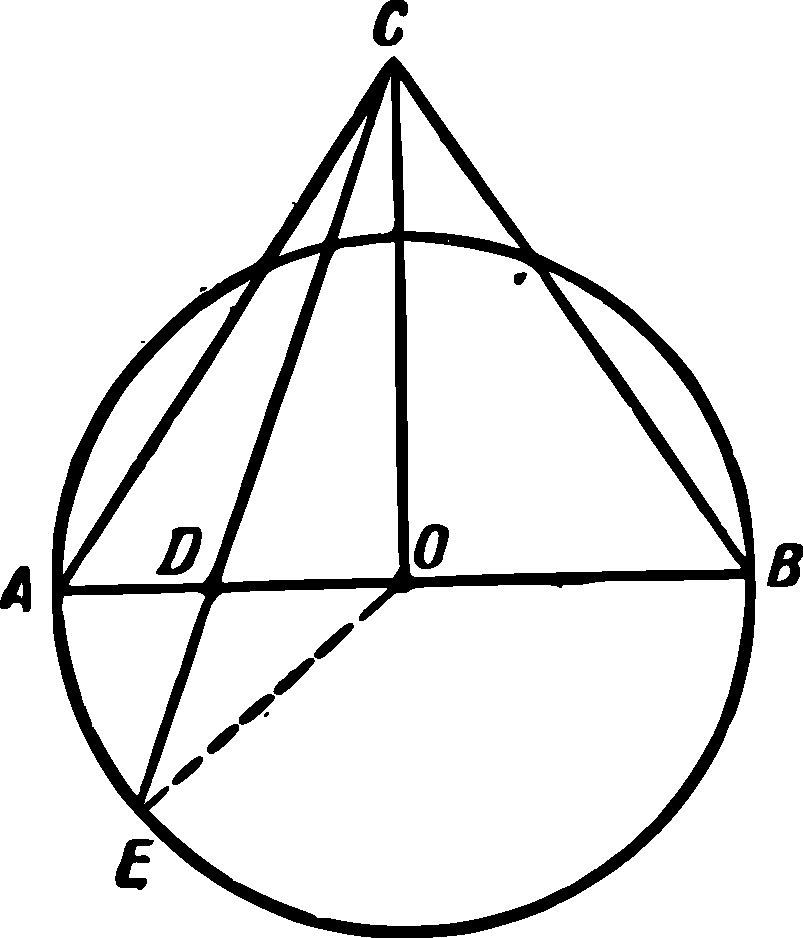
\includegraphics[width=\textwidth]{figures/ch-10/fig-149.pdf}
\sidecaption{An approximate geometric method of dividing a circle into $n$ equal parts.\label{fig-149}}
\end{marginfigure}



For example, let's say we need to divide a given circle (\figr{fig-149}) into nine equal parts. Construct a scalene triangle $ACB$ on some diameter $AB$ of the circle and divide the diameter $AB$ at point $D$ in the ratio $AD:AB = 2:9$ (generally $AD:AB = 2:n$).

Connect points $C$ and $D$ with a line segment and extend it to intersect the circle at point $E$. Then, the arc $\wideparen{AE}$ will be approximately 1/9 of the circle (generally $\wideparen{AE} = \ang{360}/n$), or chord $AE$ will be the side of a regular inscribed nonagon ($n$-gon).

The relative error in this method is about 0.8\%.


If we express the relationship between the central angle AOE, formed in the described construction, and the number of divisions \( n \), we get the following exact formula:
\begin{equation*}%
\tan \wideparen{AOE} = \frac{\sqrt{3}}{2} \cdot \frac{n^2 + 16n - 32 - n}{n - 4}
\end{equation*}
For larger values of \( n \), this can be approximated by the formula:
\begin{equation*}%
\tan \wideparen{AOE} = 4 \, \sqrt{3} \cdot \left(\frac{1}{n} - \frac{2}{n^2}\right)
\end{equation*}
On the other hand, for exact division of the circle into \( n \) equal parts, the central angle should be equal to \(\ang{360}/n \). By comparing the angle  \(\ang{360}/n \) with the angle $AOE$, we obtain the error made when considering the arc AE as \( 1/n \) part of the circle. The following table shows the error for some values of \( n \).

\begin{table*}
\centering
\begin{small}
\begin{tabular}{p{1cm}lllllllll}
\toprule
$n$	& 3	& 4	& 5	& 6	& 7	& 8	& 10	 & 20 & 60 \\
\midrule
$\ang{360}/n$ &	\ang{120} & 	\ang{90} & 	\ang{72} & 	\ang{60} & 	\ang{51;26}	& \ang{45} & \ang{36} & \ang{18} & \ang{6}\\
$\wideparen{AOE}$	&	\ang{120} & 	\ang{90} & 	\ang{71;57} & 	\ang{60} & 	\ang{51;31}	& \ang{45;11} & \ang{36;21} & \ang{18;38} & \ang{6;26}\\
Error \% & 0 & 0 & 0.07 & 0 & 0.17 & 0.41 & 0.97 &  3.5 & 7.2 \\
\bottomrule
\end{tabular}
\end{small}
\end{table*}

As can be seen from the table, this method can approximately divide the circle into 5, 7, 8, or 10 parts with a small relative error ranging from 0.07\% to 1\%, which is quite acceptable for most practical purposes. However, as the number of divisions \( n \) increases, the accuracy of the method decreases noticeably, i.e., the relative error increases, but studies show that for any \( n \), the error does not exceed 10\%.




\section[Billiard Ball Problem]{Direction of the Shot (Billiard Ball Problem)}

Hitting a billiard ball into a pocket by making it bounce off one, two, or even three rails of the table means, first of all, solving a geometric ``construction'' problem in your mind.

It's crucial to accurately ``eyeball'' the first point of impact on the rail; the subsequent path of the elastic ball on a good table will be determined by the law of reflection (\emph{the angle of incidence equals the angle of reflection}).



\begin{figure}[h!]
\centering
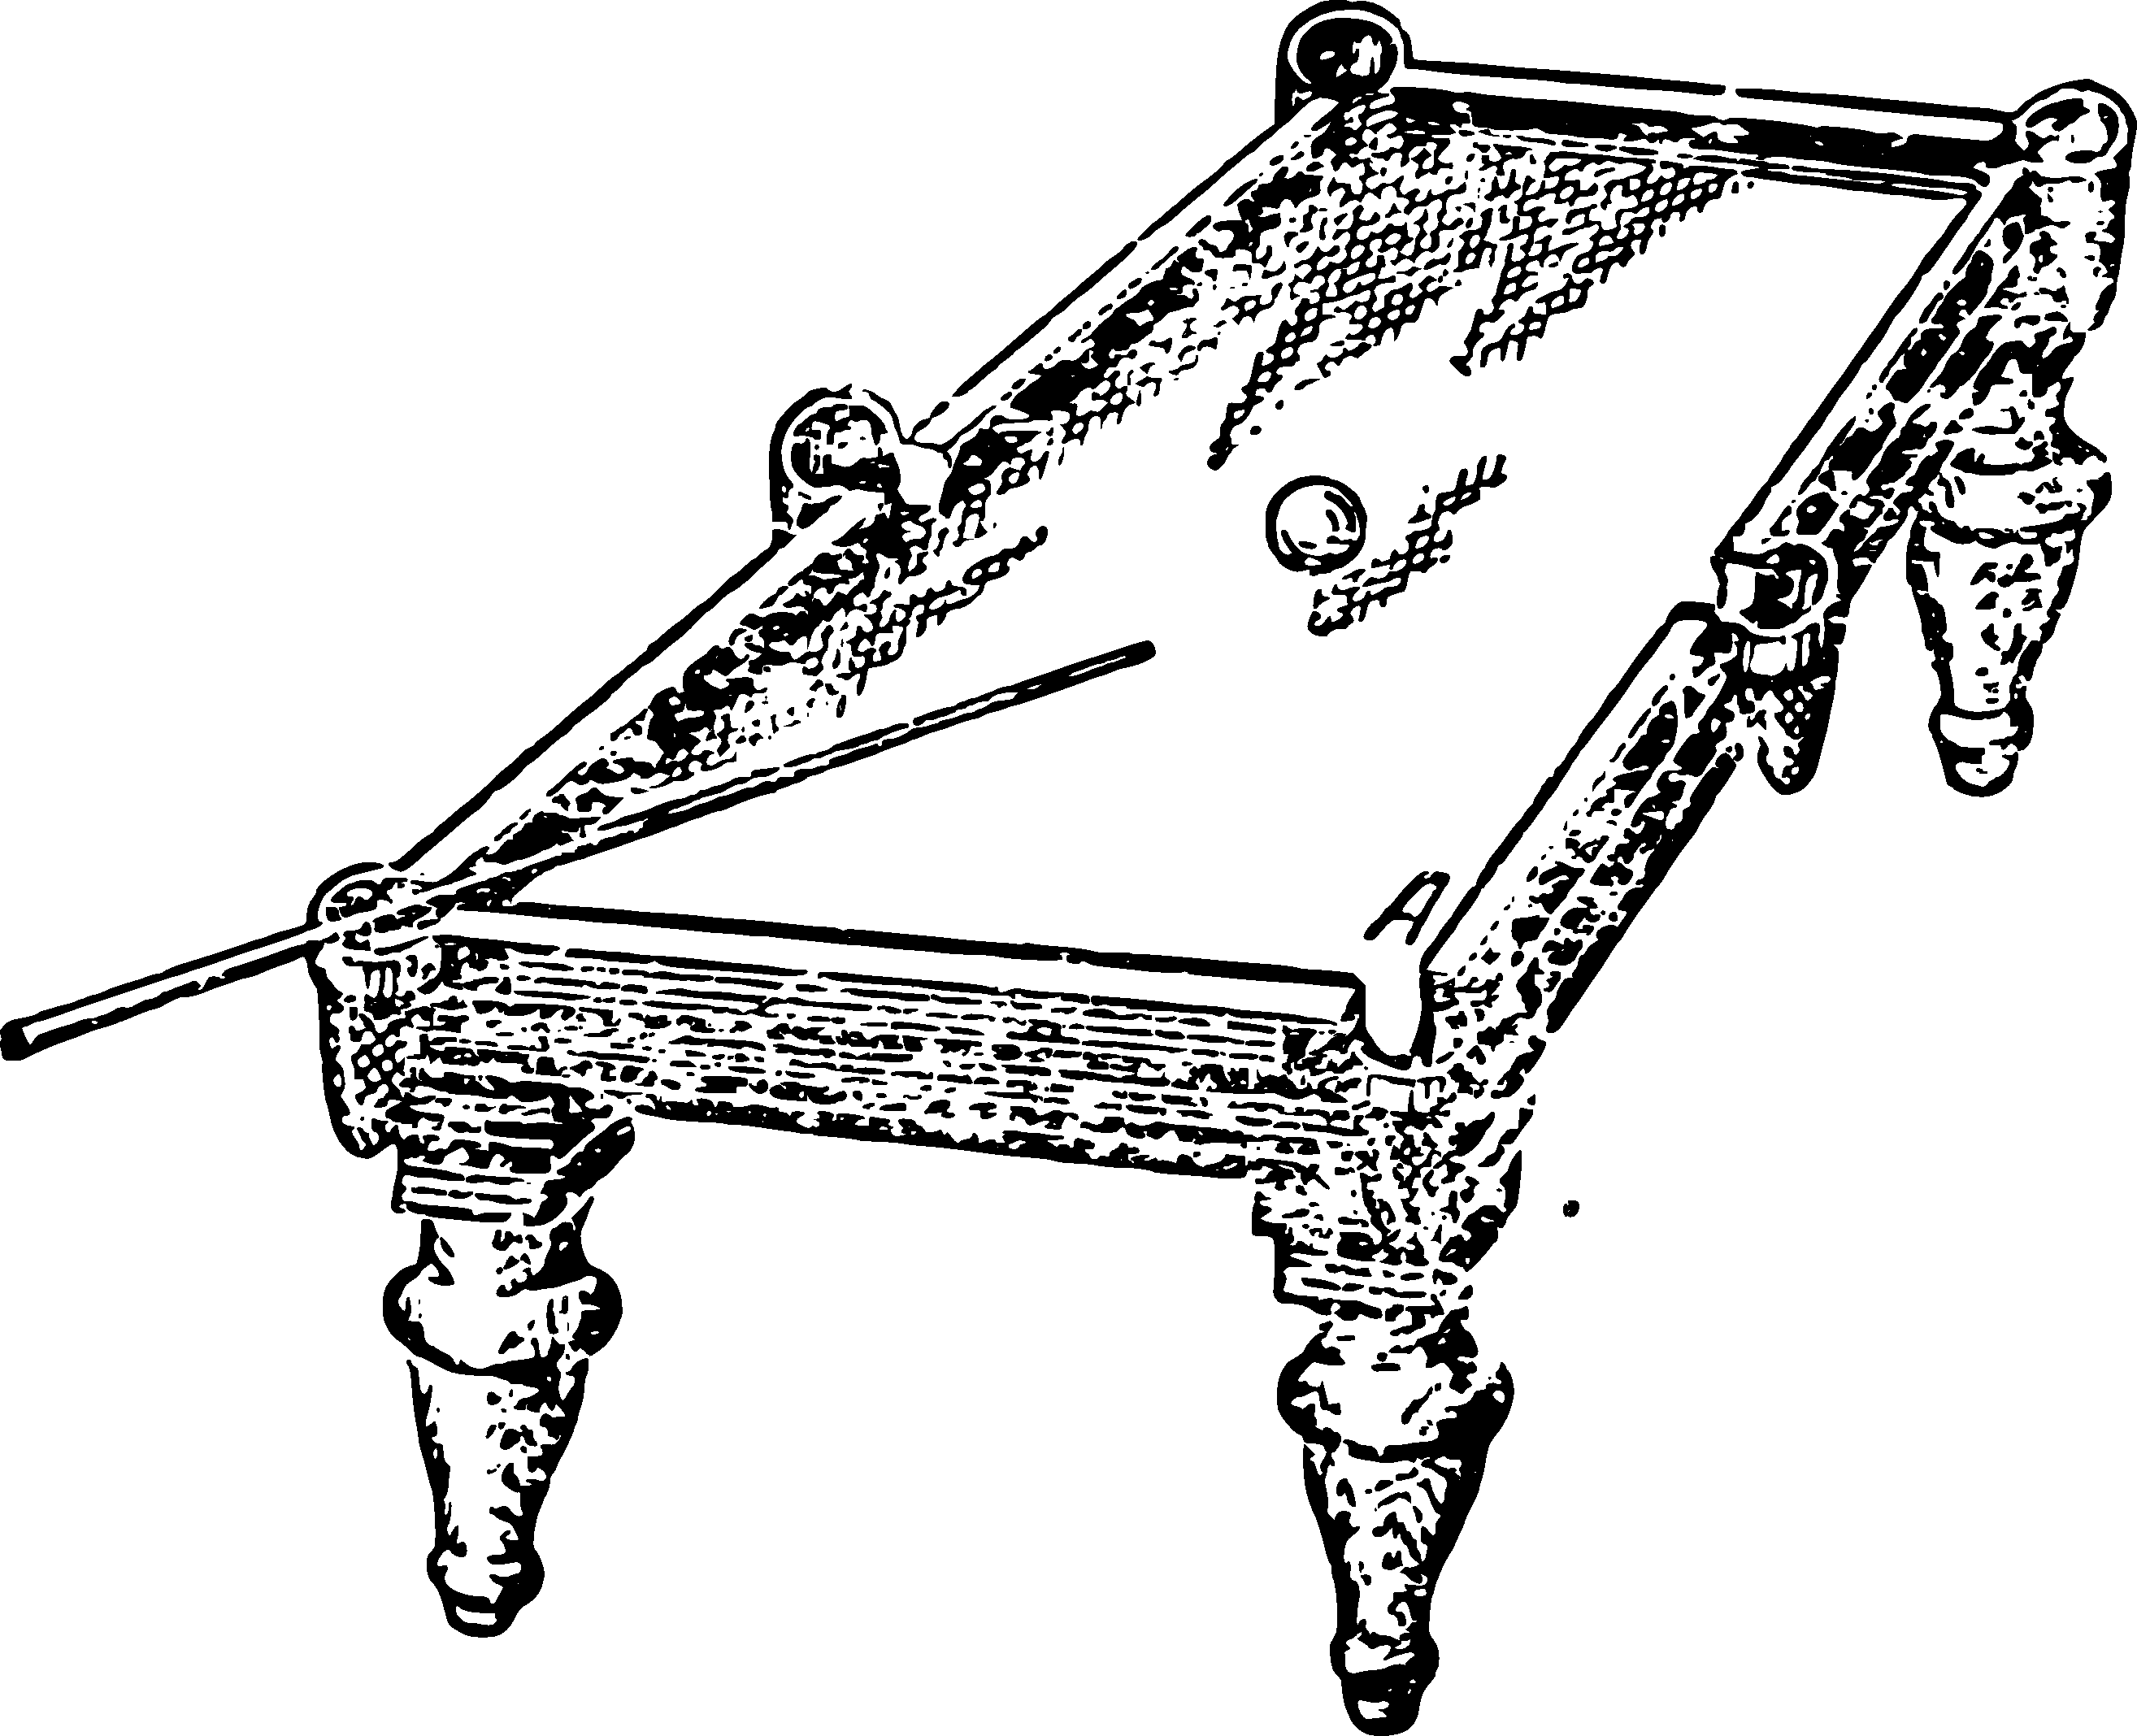
\includegraphics[width=0.7\textwidth]{figures/ch-10/fig-150.pdf}
\sidecaption{A geometric problem on a billiard table.\label{fig-150}}
\end{figure}




\ques What geometric concepts can help you find the direction of the shot so that a ball located, for example, in the middle of the billiard table, after three bounces, lands in pocket $A$? (\figr{fig-150}).


\ans You need to imagine that three more tables are placed along the short side of the billiard table, and aim in the direction of the farthest pocket on the third imaginary table.

\figr{fig-151} helps clarify this statement. Let \( OabcA \) be the path of the ball. If you flip the ``table'' $ABCD$ around $CD$ by \ang{180} degrees, it will occupy position $I$, then flip it again around $AD$ and once more around $BC$, it will occupy position $III$. As a result, pocket $A$ will be at the point marked $A_{1}$.

Based on the obvious equality of the triangles, you can easily prove that \( ab_{1} = ab \), \( b_{1}c_{1} = bc \), and \( c_{1}A_{1} = cA \), i.e., the length of the straight line \( OA_{1} \) is equal to the length of the broken line \( OabcA \).


\begin{marginfigure}%[h!]
\centering
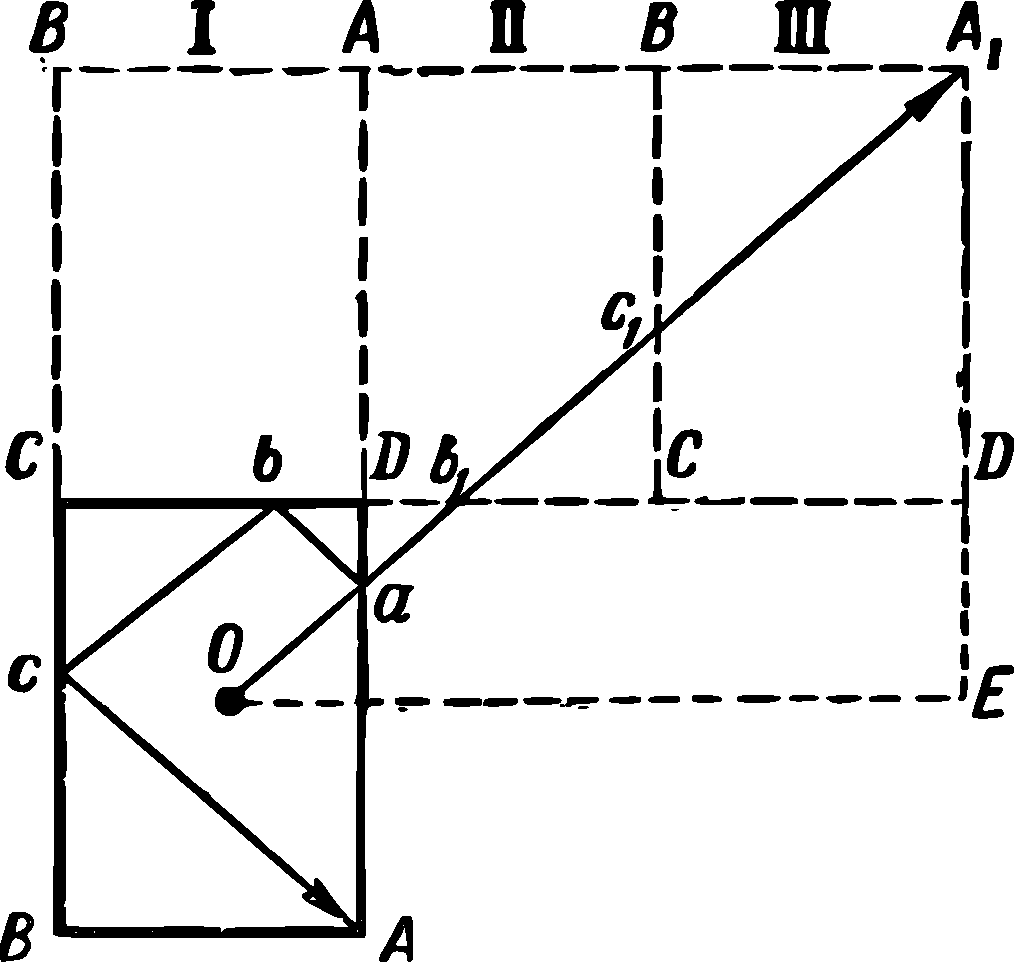
\includegraphics[width=\textwidth]{figures/ch-10/fig-151.pdf}
\sidecaption{A geometric problem on a billiard table.\label{fig-151}}
\end{marginfigure}


Therefore, aiming at the imaginary point $A_{1}$ will cause the ball to travel along the path \( OabcA \), and it will land in pocket $A$.

Let’s consider another question: under what condition will the sides \( OE \) and \( A_{1}E \) of the right triangle \( A_{1}EO \) be equal?

It is easy to establish that \( OE = 5/2 \, AB \) and \( A_{1}E = 3/2\, BC \). If \( OE = A_{1}E \), then \( 5/2 AB = 3/2\, BC \), or \( AB = 3/5 \, BC \).

Thus, if the short side of the billiard table is 3/5 of the long side, then \( OE = EA_{1} \); in this case, you can direct the shot of a ball located in the middle of the table at a \ang{45} angle to the rail.

\section{The ``Smart'' Ball}

Simple geometric constructions just helped us solve a problem involving a billiard ball. Now let's have the same billiard ball solve an interesting, old problem on its own.

Is that even possible? -- A ball can't think. True, but when a calculation needs to be performed, and we know the operations and their order, such a calculation can be entrusted to a machine, which will perform it quickly and without error.

Many mechanisms have been invented for this purpose, from simple mechanical calculators to complex electronic machines.

In leisure time, people often entertain themselves with the problem of how to pour a specific amount of water from a filled container of known capacity using two other empty containers, also of known capacities.

Here is one of many problems of this kind:

Divide the contents of a 12-bucket barrel in half using two empty barrels of nine buckets and five buckets.

To solve this problem, you don’t need to experiment with actual barrels. All necessary ``pourings'' can be done on paper with a simple scheme:

%\begin{table*}

\begin{small}
\centering
\begin{tabular}{@{}r *{9}{c}@{}}
\toprule
9 Buckets & 0 & 7\tikzmark{a3} & 7\tikzmark{a6} & 2 & 2\tikzmark{a9} & 0 & 9\tikzmark{a11} & 6 & 6 \\
5 Buckets & 5\tikzmark{a2} & 5\tikzmark{a4} & 0 & 5\tikzmark{a7} & 0 & 2\tikzmark{a10} & 2 & 5\tikzmark{a12} & 0 \\
12 Buckets\tikzmark{a1} & 7 & 0 & 5\tikzmark{a5} & 5 & 
   \makebox[\widthof{0}][c]{10}\tikzmark{a8} & 
   \makebox[\widthof{0}][c]{10} & 
   1 & 1 & 6\tikzmark{a13} \\ 
\bottomrule
\end{tabular}
\end{small}
%\end{table*}
\begin{tikzpicture}[overlay, remember picture, 
  shorten >=8pt, 
  shorten <=3pt, 
  transform canvas={yshift=.33\baselineskip}]
    \draw [-stealth, red, thick] ({pic cs:a1}) -- ({pic cs:a2});
    \draw [-stealth, red, thick] ({pic cs:a2}) -- ({pic cs:a3});
    \draw [-stealth, red, thick] ({pic cs:a4}) -- ({pic cs:a5});
    \draw [-stealth, red, thick] ({pic cs:a6}) -- ({pic cs:a7});
    \draw [-stealth, red, thick] ({pic cs:a7}) -- ({pic cs:a8});
    \draw [-stealth, red, thick] ({pic cs:a9}) -- ({pic cs:a10});
    \draw [-stealth, red, thick] ({pic cs:a10}) -- ({pic cs:a11});
    \draw [-stealth, red, thick] ({pic cs:a11}) -- ({pic cs:a12});
    \draw [-stealth, red, thick] ({pic cs:a12}) -- ({pic cs:a13}); 
\end{tikzpicture}

% https://tex.stackexchange.com/questions/718439/aligning-arrows-in-table

In each column, record the result of the current pouring. 

Fill the five-bucket barrel. The nine-bucket barrel is empty (0), and seven buckets remain in the 12-bucket barrel. 

Pour the seven buckets from the 12-bucket barrel into the nine-bucket barrel, and so on.

The scheme has nine columns, indicating that nine pourings were needed to solve the problem.

Try to find your own solution to the proposed problem, establishing a different order of pourings.

After several attempts, you will undoubtedly succeed, as the proposed pouring scheme is not the only possible one; however, with a different order of pourings, you might need more than nine.

In this context, it is interesting to explore the following:

1. Can a specific order of pourings be established that can be followed in all cases, regardless of the capacities of the containers?
2. Can any possible amount of water be poured from a third container using two empty containers, e.g., for example, from a 12-bucket barrel using barrels in 9 and 5 buckets, one bucket of water, or two buckets, or three, four, etc. to 11?

The ``smart'' ball will answer all these questions if we now construct a special ``billiard table'' for it.

Draw a sheet of paper in a slant grid so that the cells are equal rhombuses with acute angles of \ang{60}, and construct the figure $OABCD$ as shown in Fig. 152.

This will be the "billiard table." If you push the billiard ball along OD, it will bounce off the rail AD exactly according to the law "the angle of incidence equals the angle of reflection" (/ OAM = / MAC), and the ball will roll along the straight line AC, connecting the vertices of the small rhombuses; it will bounce at point C from...

\begin{center}
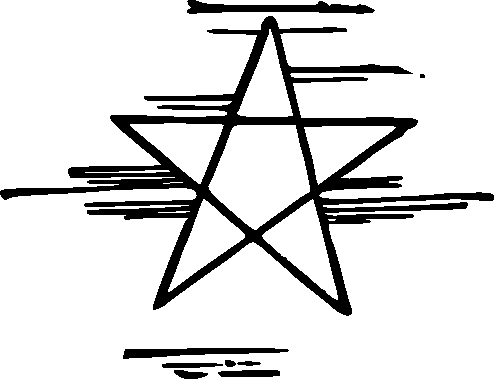
\includegraphics[width=0.3\textwidth]{figures/ch-10/fig-ch-10-tail.pdf}
\end{center}


















